\documentclass[14pt]{article}

\usepackage[utf8]{inputenc}
\usepackage[T2A]{fontenc}
\usepackage[english,russian]{babel}

\usepackage{graphicx}
\usepackage{amsmath}

\usepackage{hyperref}

\usepackage[normalem]{ulem}  % для зачекивания текста

%\usepackage{natbib}		% библиография

%\usepackage{algorithm2e}	% Алгоритмы

\begin{document}

\title{Расчёт градиентов акфифера}	
\maketitle

\section{Обозначения}
 	\begin{align*}
		& \alpha - \text{фаза}\\
		& p \equiv p_{o} - \text{давление, при присутствии капелярных сил - давление нефти} 
 	\end{align*}
 	
	intrinsic modulus/parament -- свойственный/собственный модель/параметр
\section{Модель} 

\begin{equation} \label{fil}
	\nabla\sigma\nabla p = c \cdot h \frac{dp}{dt}+\delta(x,y)
\end{equation}


\begin{equation} \label{bc}
\delta(x,y)  = \left\{\begin{array}{crl}
0, \;при\;(x,y) \notin\ \Gamma_{in}\cup\Gamma_{out}\\
q_j, \;при\;(x,y) \in \Gamma_{in}\\
q_{aq}, \;при\;(x,y) \in \Gamma_{out}
\end{array}\right.,
\end{equation}
\begin{equation*}
p = p_0\mbox{,\quad при $t=0$},
\end{equation*}
где $\sigma$ - гидропроводность, $p$ - пластовое давление, $c$ - эффективная сжимаемость, $h$ - эффективная толщина, $q_j$ - расход жидкости в $j$ скважине, $\Gamma_{in}$ - множество координат источников/стоков (скважин), $\Gamma_{out}$ - внешняя граница, $p_0$ - пластовое давление в начальный момент времени $t=0$, $q_{aq}$ - удельный расход жидкости через внешнюю границу.
Гидропроводность $\sigma$ находится по формуле:
\begin{equation} \label{sig}
	\sigma = a \sigma_0+b,
\end{equation}
где $\sigma_0$ - исходная гидропроводность, $a$ и $b$ - поправочные коэффициенты.

Для замыкания уравнений (\ref{fil}) - (\ref{bc}) используется модель водоносного контура, которую в общем виде можно представить в виде: 
\begin{equation} \label{f_aq}
F(p_{aq}, p,\boldsymbol{\nu})=0,
\end{equation}
где $\boldsymbol{\nu}$ - набор настраиваемых параметров водоносного контура, состав которого зависит от сложности модели. В Дальнейших расчётах и выкладках будет использована одна из 4-х моделей - модель аквифера конечного объёма \cite{dake},\cite{fet}.Эта модель позволяет описать изменение давления $p_{aq}$ в аквифере имеющем конечный объём и связанный с нефтяным пластом. 
\begin{equation} \label{aq_analit}
F(p_{aq}, p,\boldsymbol{\nu})=c_{aq}V_{aq}\frac{dp_{aq}}{dt} - \lambda\oint_{\Gamma_{out}}\frac{\sigma}{h}(p-p_{aq})dl = 0,
\end{equation}
где $V_{aq}$ - объём аквифера. Модель имеет 2 настраиваемых параметра, $\boldsymbol{\nu} = [\lambda, V_{aq}]$.

\section{Конечно-разностная форма} 
При численном решении уравнение \ref{fil} записывается в матричном виде:
\begin{equation} \label{fil_fin_def}
\boldsymbol{A}\boldsymbol{p}^n = \boldsymbol{\beta}\circ\boldsymbol{p}^{n-1} - \boldsymbol{q}^n - \lambda \cdot \boldsymbol{s}\circ\boldsymbol{\sigma}\circ (\boldsymbol{p}^{n-1}-p_{aq}^{n-1}),
\end{equation}
где $\boldsymbol{A}$ - разреженная диагональная матрица коэффициентов, $ \boldsymbol{p}^n $ - массив значений пластового давления, $ n $ номер временного шага $ n=1:N_t $,  $ N_t $ - количество временных шагов, $ \boldsymbol{q}^n $ - массив значений расхода жидкости на скважинах, $ \boldsymbol{s} $ - массив значений описывающий контакт разностных ячеек с границей, значения равны 0 для ячеек не имеющих контакта с аквифером и не равны 0 для ячеек контактирующих с аквифером, элементы массив $ \boldsymbol{\beta} $ находится из формулы:

\begin{equation} \label{beta_init}
 \beta_i = \frac{c {V_p}_i}{\bigtriangleup t},
\end{equation} 
где $ {V_p}_i $ - объём пор $ i $ - той ячейки, ${\bigtriangleup t}$ - шаг по времени.
Матрицу $\boldsymbol{A}$ для дальнейших преобразований удобно представить в виде:
\begin{equation} \label{A_diag}
\boldsymbol{A} = \boldsymbol{A_t} - diag\left(\boldsymbol{w}_0\right) - diag\left(\boldsymbol{\beta}\right),
\end{equation}
где $ \boldsymbol{A_t} $ - диагональная матрица проводимостей (нижний индекс $ "t" $ -transmissibility), $ diag\left(\boldsymbol{w}_0\right) $ - диагональная матрица продуктивностей скважины, $ diag\left(\boldsymbol{\beta}\right) $ - диагональная матрица описывающая "упругоёмкость" породы. Массив $\boldsymbol{w}_0$ содержит продуктивности скважин, значения равны 0 если через ячейку не проходит ни одной скважины. Продуктивность скважины рассчитывается по формуле Дюпюи:
\begin{equation} \label{WI}
w = 2 \pi\frac{\sigma}{ln\left(\frac{R_k}{r_w}\right)},
\end{equation} 
где $ R $ - приведенный радиус ячейки, $ r_w $ - радиус скважины.

Модель "аквифера конечного объёма" в конечно-разностной форме в явном виде по времени можно записать следующим образом сделав замену (\ref{beta_init}): 
\begin{equation} \label{aq_num}
c_{aq} V_{aq}\frac{p_{aq}^n - p_{aq}^{n-1}}{\bigtriangleup t} = 
\beta_{aq}(p_{aq}^n - p_{aq}^{n-1}) =  
\lambda\sum_{i \in bnd}s_i\sigma_i(p_i^{n-1}-p_{aq}^{n-1}),
\end{equation}
где $ i $ - номер ячейки, $bnd$ - множество индексов граничных ячеек.

\section{Обратная задача}
Обратная задача решается в оптимизационной постановке, которая заключается в минимизации целевой функции $J$, в качестве которой выступает "mean squared error" (MSE). Аргументами целевой функции выступают фактические (замеренные) и расчётные значения пластового давления в точках расположения скважин в заданные моменты времени. Целевая функция характеризует отклонение расчётных и фактических значений давления и записывается следующим образом:
\begin{equation} \label{mse}
J=\frac{1}{N}\sum_{i=1}^N{\left(p_f^i-p_c^i\right)^2}
\end{equation}
где $p_c^i$ -расчетное значение пластового давления, $p_f^i$ - фактическое значение, $i$ - номер замера, $N$ - количество замеров. Решение задачи можно искать при использовании градиентного оптимизационного алгоритма. Решение заключается в определении набора параметров модели соответствующих минимуму $J$ и удовлетворяющих ограничениям в виде неравенств:
\begin{equation} \label{ubnd}
u_{k\;min}\leq\ u_k\leq u_{k\;max}, \quad u_k \in \boldsymbol{u},
\end{equation}
где $u_{k\;min}$ и $u_{k\;max}$ - минимальный и максимальные значения для каждого параметра. Помимо ограничения на управляющие параметры необходимо учитывать физические или экспертные ограничения на значения фазовых переменных (давлений). Так к примеру физическим нижним ограничением для значения давления является 0. В качестве верхнего ограничения может выступать значение максимально допустимое давление для насосов нагнетательных скважин или некоторая другая экспертная оценка максимально возможного давления. Ввиду особенности получаемого решения (уравнения Лапласа), минимальные и максимальные значения фазовых переменных получаются в ячейках в которых находятся активные (работающие) скважины, таким образом для учёта ограничений фазовых переменных можно контролировать только эти значения. Для учёта ограничения на фазовые переменные добавим в целевой функционал (\ref{mse}) штрафную функцию и получим: 
\begin{equation} \label{mse_bnd_p}
J=\frac{1}{N}\sum_{i=1}^N{\left(p_f^i-p_c^i\right)^2} + \sum_{k=1}^K{f_{SP}(p_{min} - p^k_c)} + \sum_{k=1}^K{f_{SP}(p^k_c-p_{max})},
\end{equation}
где $ p_{min} $ и $ p_{max} $ минимальное и максимальное ограничение на значение пластового давления соответственно, $K$ - количество расчетных значений пластового давления в ячейках с работающими скважинами,  $f_{SP}$ - функция активации "SoftPlus" \cite{Glorot2011}, которая записывается следующим образом:
\begin{equation} \label{SP}
f_{SP}(x) = \ln\left(1+e^{\alpha x}\right),
\end{equation}
производная 
\begin{equation} \label{dSP}
f'_{SP} = \frac{\alpha}{1+e^{-\alpha x}},
\end{equation}
где $ \alpha $ - масштабирующий коэффициент, при изменении которого можно регулировать степень влияния штрафной функции. Функция "SoftPlus" является гладкой и дифференцируемой, для всей области определения, что хорошо подходит для градиентных методов оптимизации. 

При использовании градиентного метода оптимизации, необходимо найти компоненты градиента целевой функции, которые можно записать в следующем виде:
\begin{multline}\label{dJ_du}
	\frac{\partial J}{\partial u_k} = \frac{1}{N}\sum_{i=1}^N \left(p_f^i-p_c^i\right)\frac{\partial p_c^i}{\partial u_k} - \sum_{k=1}^K{f'_{SP}(p_{min} - p^k_c)\frac{\partial p_c^k}{\partial u_k}} + {} \\ {}
	 + \sum_{k=1}^K{f'_{SP}(p^k_c-p_{max})\frac{\partial p_c^k}{\partial u_k}}.
\end{multline}
Для решения оптимизационной задачи ($ J \rightarrow min $) необходимо чтобы каждая компонента градиента целевой функции стремилась к 0, что можно записать как:
\begin{equation} \label{dJ_du0}
\frac{\partial J}{\partial u_k} \rightarrow 0
\end{equation}
Как видно из (\ref{dJ_du}) для расчёта компонент градиента необходимо найти значения производных пластового давления от управляющих параметров. Также стоит сделать замечание о том, что использование дополнительных ограничений на значения фазовых переменных имеет смысл в случае если множество фактических замеров намного меньше множества индексов работающих скважин на для которых необходимо рассчитывать значения пластового давления. 

\section{Нахождение компонент градиента}
Основную сложность составляет нахождение компонент градиента целевой функции. Найдём их численно при использовании уравнений (\ref{fil_fin_def}) и (\ref{aq_num}). В качестве управляющих параметров $ u_k $ выступают коэффициенты $ a $ и $ b $ используемые в корректировке значений гидропроводности   (\ref{sig}), коэффициент продуктивности аквифера $ \lambda $ и поправочный коэффициент для порового объёма аквифера $ \gamma $. Коэффициент $ \gamma $ позволяет записать искомый объём как:
\begin{equation*} \label{gamma_init}
V_{aq} = \gamma{V_0}_{aq},
\end{equation*}
 где $ {V_0}_{aq}$ -  исходное значения порового объёма и $ \gamma $ - коэффициент (множитель) на исходный поровый объём, тогда используя {\ref{beta_init}}, получим:
 \begin{equation} \label{beta_gamma}
 \beta_{aq} = \gamma {\beta_0}_{aq},
 \end{equation}
  Таким образом вектор управляющих параметров $ \boldsymbol{u} = [a,b,\lambda,\gamma]$, найдём значения производных давления по управляющим параметрам, при продифференцируем уравнение (\ref{fil_fin_def}), в общем виде получим:

\begin{multline} \label{dFP_du}
\frac{\partial \boldsymbol{A}}{\partial u_k}\boldsymbol{p}^n + \boldsymbol{A}\frac{\partial \boldsymbol{p}^n}{\partial u_k} =
\boldsymbol{\beta}\circ\frac{\partial \boldsymbol{p}^{n-1}}{\partial u_k} + \frac{\partial \lambda}{\partial u_k}\boldsymbol{\sigma}\circ(\boldsymbol{p}^{n-1}-p_{aq}^{n-1})+ {} \\
{} + 
\lambda\frac{\partial \boldsymbol{\sigma}}{\partial u_k}\circ(\boldsymbol{p}^{n-1}-p_{aq}^{n-1})+
\lambda\boldsymbol{\sigma}\circ\left(\frac{\partial \boldsymbol{p}^{n-1}}{\partial u_k}-\frac{\partial p_{aq}^{n-1}}{\partial u_k}\right),
\end{multline}
где $ \frac{\partial \boldsymbol{A}}{\partial u_k} $ - разреженная матрица, $ \frac{\partial \boldsymbol{p}^n}{\partial u_k} $ - искомый вектор, который можно найти решив СЛАУ преобразовав уравнение к виду "$\textbf{A}\textbf{x}=\textbf{b}$".

Продифференцировав уравнение (\ref{aq_num}) получим
\begin{eqnarray} \label{dFAq_num}
\frac{\partial \beta_{aq}}{\partial u_k}\left(p_{aq}^n - p_{aq}^{n-1}\right)
+\beta_{aq}\left(\frac{\partial p_{aq}^n}{\partial u_k} - \frac{\partial p_{aq}^{n-1}}{\partial u_k}\right)
 = \frac{\partial \lambda}{\partial u_k}\sum_{i \in bnd}s_i\sigma_i\left(p_i^{n-1}-p_{aq}^{n-1}\right)+ {} \nonumber\\
 {} + \lambda\sum_{i \in bnd}s_i\frac{\partial \sigma_i}{\partial u_k}\left(p_i^{n-1}-p_{aq}^{n-1}\right)+
 \lambda\sum_{i \in bnd}s_i\sigma_i\left(\frac{\partial p_i^{n-1}}{\partial u_k}-\frac{\partial p_{aq}^{n-1}}{\partial u_k}\right).
\end{eqnarray}
Используя уравнение (\ref{dFP_du}) запишем уравнения для нахождения значения производных по давлению для каждого управляющего параметра. Первым найдем уравнения для поправок на значения гидропроводности $ a $ и $ b $ из уравнения (\ref{sig}). Помимо фазовых переменных (давления) и непосредственно самой гидропроводности от управляющих параметров $ a $ и $ b $ зависит матрица $ \boldsymbol{A} $. Для удобства матрицу $ \boldsymbol{A} $ запишем в виде суммы матриц (\ref{A_diag}), значения гидропроводности используется только в слагаемых отвечающих за проводимость между ячейками и продуктивность скважин, таким образом матрицу содержащую производные по эементов матрицы по управляющим параметрам можно записать следующим образом:
\begin{equation} \label{dA_du_k}
\frac{\partial \boldsymbol{A}}{du_k} = \frac{\partial \boldsymbol{A_t}}{\partial u_k}-diag(\frac{\partial \boldsymbol{w_0}}{\partial u_k})
-diag(\frac{\partial \boldsymbol{\beta}}{\partial u_k}).
\end{equation}
Каждый элемент матрицы $ \boldsymbol{A_t} $ рассчитывается по формуле:
\begin{equation} \label{Tij}
T_{i,j} = \frac{2{\sigma_i}{\sigma_j}}{{\sigma_i} + {\sigma_j}}
\end{equation}
Производную проводимости между $ i $-той и $ j $-той ячейками $ T_{ij} $ по управляющим параметрам можно записать следующим образом:
\begin{equation} \label{dTij_da}
\frac{\partial T_{i,j}}{\partial u_k} = \frac{\partial T_{i,j}}{\partial \sigma_i}\frac{\partial \sigma_i}{\partial u_k} + \frac{\partial T_{i,j}}{\partial \sigma_j}\frac{\partial \sigma_j}{\partial u_k}
\end{equation}
Множитель вида $ \frac{\partial T_{i,j}}{\partial \sigma_i} $ находится по формуле:
\begin{equation} \label{dTij_dsigma_i}
\frac{\partial T_{i,j}}{\partial \sigma_i} = 2\left(\frac{\sigma_j}{{\sigma_i} + {\sigma_j}}\right)^2
\end{equation}

Массив множителей $ \frac{\partial \sigma_i}{\partial u_k} $ при $ u_k \in [a,b]$ и учётом (\ref{sig}) записывается в виде:
\begin{equation*} \label{dsig_da}
\frac{\partial \boldsymbol{\sigma}}{\partial a} = \boldsymbol{\sigma_0},
\end{equation*}
\begin{equation*} \label{dsig_db}
\frac{\partial \boldsymbol{\sigma}}{\partial b} = \boldsymbol{e},
\end{equation*}
где $ \boldsymbol{e} $ - массив размера равного количеству ячеек, каждый элемент которого равен 1.
Элементы матрицы $ diag(\frac{\partial \boldsymbol{w_0}}{\partial u_k}) $ находятся по формуле:
\begin{equation} \label{dWI}
\frac{\partial w_i}{\partial u_k} = \frac{\partial w_i}{\partial \sigma_i}\frac{\partial \sigma_i}{\partial u_k} =  \frac{2 \pi}{ln\left(\frac{R_k}{r_w}\right)}\frac{\partial \sigma_i}{\partial u_k}.
\end{equation} 
Матрица $ diag(\frac{\partial \boldsymbol{\beta}}{\partial u_k}) $ при $ u_k \in [a,b]$ нулевая. Приведем уравнение (\ref{dFP_du})к виду "$\textbf{A}\textbf{x}=\textbf{b}$" при $u = a,b,\lambda,\gamma$:

\begin{multline} \label{eq_dp_da}
\boldsymbol{A}\frac{\partial \boldsymbol{p}^n}{\partial a} = \boldsymbol{\beta}\frac{\partial\boldsymbol{p}^{n-1}}{\partial a}
+ \lambda\boldsymbol{\sigma_0} \circ \left(\boldsymbol{p}^{n-1}-p_{aq}^{n-1}\right) +  {} \\
{} +\lambda\boldsymbol{\sigma} \circ \left(\frac{\partial \boldsymbol{p}^{n-1}}{\partial a}-\frac{\partial p_{aq}^{n-1}}{\partial a}\right)
-\frac{\partial \boldsymbol{A}}{\partial a}\boldsymbol{p}^n,
\end{multline}

\begin{multline} \label{eq_dp_db}
\boldsymbol{A}\frac{\partial \boldsymbol{p}^n}{\partial b} = \boldsymbol{\beta}\frac{\partial\boldsymbol{p}^{n-1}}{\partial b} + \lambda(\boldsymbol{p}^{n-1}-p_{aq}^{n-1}) +  {} \\
{} + \lambda\boldsymbol{\sigma} \circ \left(\frac{\partial \boldsymbol{p}^{n-1}}{\partial b}-\frac{\partial p_{aq}^{n-1}}{\partial b}\right)
-\frac{\partial\boldsymbol{A}}{\partial b}\boldsymbol{p}^n,
\end{multline}

\begin{equation} \label{eq_dp_dlam}
\boldsymbol{A}\frac{\partial \boldsymbol{p}^n}{\partial \lambda}
 = \beta\frac{\partial \boldsymbol{p}^{n-1}}{\partial \lambda} + \sigma \circ \left(\boldsymbol{p}^{n-1}-p_{aq}^{n-1}\right)
 +\lambda\sigma \circ \left(\frac{\partial \boldsymbol{p}^{n-1}}{\partial \lambda}
 -\frac{\partial p_{aq}^{n-1}}{\partial \lambda}\right)
\end{equation}

При учёте (\ref{beta_gamma}) запишем уравнение для нахождения производной пластового давления по параметру $ \gamma $.
\begin{equation} \label{eq_dp_dgamma}
\boldsymbol{A}\frac{\partial \boldsymbol{p}^n}{\partial \gamma} =
 \beta\frac{\partial \boldsymbol{p}^{n-1}}{\partial \gamma}
  + \lambda\sigma \circ \left(\frac{\partial \boldsymbol{p}^{n-1}}{\partial \gamma}
  -\frac{\partial p_{aq}^{n-1}}{\partial \gamma}\right)
\end{equation}


Для замыкания уравнений (\ref{eq_dp_da} - \ref{eq_dp_dgamma}) необходимо выразить производную давления в аквифере от управляющих параметров. Запишем уравнение \ref{dFAq_num} для всех управляющих параметров.

\begin{multline} \label{dAQ_da}
\frac{\partial p_{aq}^n}{\partial a}
= \frac{\lambda}{\gamma{\beta_0}_{aq}}\sum_{i \in bnd}s_i{\sigma_0}_i\left(p_i^{n-1}-p_{aq}^{n-1}\right) +  {} \\
{} +\frac{\lambda}{\gamma{\beta_0}_{aq}}\sum_{i \in bnd}s_i\sigma_i\left(\frac{\partial p_i^{n-1}}{\partial a}-\frac{\partial p_{aq}^{n-1}}{\partial a}\right)+ \frac{\partial p_{aq}^{n-1}}{\partial a},
\end{multline}

\begin{multline} \label{dAQ_db}
\frac{\partial p_{aq}^n}{\partial b}
= \frac{\lambda}{\gamma{\beta_0}_{aq}}\sum_{i \in bnd}s_i \left(p_i^{n-1}-p_{aq}^{n-1}\right) +  {} \\
{} +\frac{\lambda}{\gamma{\beta_0}_{aq}}\sum_{i \in bnd}s_i\sigma_i\left(\frac{\partial p_i^{n-1}}{\partial b}-\frac{\partial p_{aq}^{n-1}}{\partial b}\right) + \frac{\partial p_{aq}^{n-1}}{\partial b},
\end{multline}

\begin{multline} \label{dAQ_dlam}
\frac{\partial p_{aq}^n}{\partial \lambda}
= \frac{\lambda}{\gamma{\beta_0}_{aq}}\sum_{i \in bnd}s_i\sigma_i\left(p_i^{n-1}-p_{aq}^{n-1}\right) +  {} \\
{} +
\frac{\lambda}{\gamma{\beta_0}_{aq}}\sum_{i \in bnd}s_i\sigma_i\left(\frac{\partial p_i^{n-1}}{\partial \lambda}-\frac{\partial p_{aq}^{n-1}}{\partial \lambda}\right)+ \frac{\partial p_{aq}^{n-1}}{\partial \lambda}.
\end{multline}
С учётом (\ref{beta_init}) запишем $ \beta_{aq} = \gamma{\beta_0}_{aq} $ и производная по продуктивности будет выглядеть следующим образом:

\begin{multline} \label{dAQ_dgamma}
\frac{\partial p_{aq}^n}{\partial \gamma} 
= \frac{\lambda}{\gamma{\beta_0}_{aq}}\sum_{i \in bnd}s_i\sigma_i\left(\frac{\partial p_i^{n-1}}{\partial \gamma}-\frac{\partial p_{aq}^{n-1}}{\partial \gamma}\right)  -  {} \\
{} - \frac{1}{\gamma}\left(p_{aq}^n - p_{aq}^{n-1}\right)
+ \frac{\partial p_{aq}^{n-1}}{\partial \gamma}.
\end{multline}
Уравнения (\ref{eq_dp_da} - \ref{dAQ_dgamma}) позволяют рассчитать значения производных пластового давления по управляющим параметрам. 

\section{Алгоритм расчёта}
Решение обратной задачи (\ref{mse_bnd_p}) находится численно методом градиентного спуска. На каждой итерации решается прямая (\ref{fil}-\ref{f_aq}) и сопряженная (\ref{eq_dp_da} - \ref{eq_dp_dgamma}) задачи. При решении которых происходит расчет показателей разработки, значений производных пластового давления по управляющим параметрам и слагаемых для расчёта компонент градиента  целевой функции. Процесс поиска решения задачи можно представить в виде следующего алгоритма:

\begin{enumerate} 
	\item Задаются начальные приближения по управляющим параметрам $ \boldsymbol{u}  = \boldsymbol{u_0}$, номер итерации k:=1;
	\item \label{list_1_2}Решается прямая и сопряжённая задачи:
	\begin{enumerate}
		\item \label{list_2_a} Для $ n=0 $, задаются начальные условия для пластового давления, значения производных давления по управляющим параметрам равны 0;
		\item Для $ n=1:N_t $ последовательно рассчитываются значения фазовых переменных и параметров разработки, значения производных пластового давления по управляющим параметрам и слагаемые компонента градиента целевой функции;
		\item Расчет значений целевой функции $ J_k $;
	\end{enumerate}
	\item Проверка критериев остановки, если выполняется выход, иначе далее;
	\item Рассчитывается при помощи значений компонент градиента целевой функции вектор управляющих параметров $ u_k $, $k := k+1$
	\item Проверка полученных управлений на предмет удовлетворения ограничениям (\ref{ubnd})
	\item Переходим к п.2
\end{enumerate}

В процессе решения на каждом временном шаге первым находится прямое решение, после чего находится сопряженное решение. При допущении стационарного состояния в начальный момент, можно предположить отсутствие влияния управляющих параметров на начальные условия, следовательно в начальный момент времени $ n=0 $  п.\ref{list_2_a} значения производных давления по управляющим параметрам равны 0:
\begin{equation*}
\frac{d\boldsymbol{p}^0}{d\gamma} = \frac{d\boldsymbol{p}^0}{d\lambda} = \frac{d\boldsymbol{p}^0}{da} = \frac{d\boldsymbol{p}^0}{db} = 0
\end{equation*}
\begin{equation*}
\frac{p_{aq}^0}{d\gamma} = \frac{p_{aq}^0}{d\lambda} = \frac{p_{aq}^0}{da} = \frac{p_{aq}^0}{db} = 0
\end{equation*}

Таким образом для нахождения на первом (и последующих) временном шаге значений производных давления необходимо знать значения фазовых переменных с текущего и предыдущего, временного шагов, а также значния производных с предыдущего временного шага.

\begin{figure}
	\center{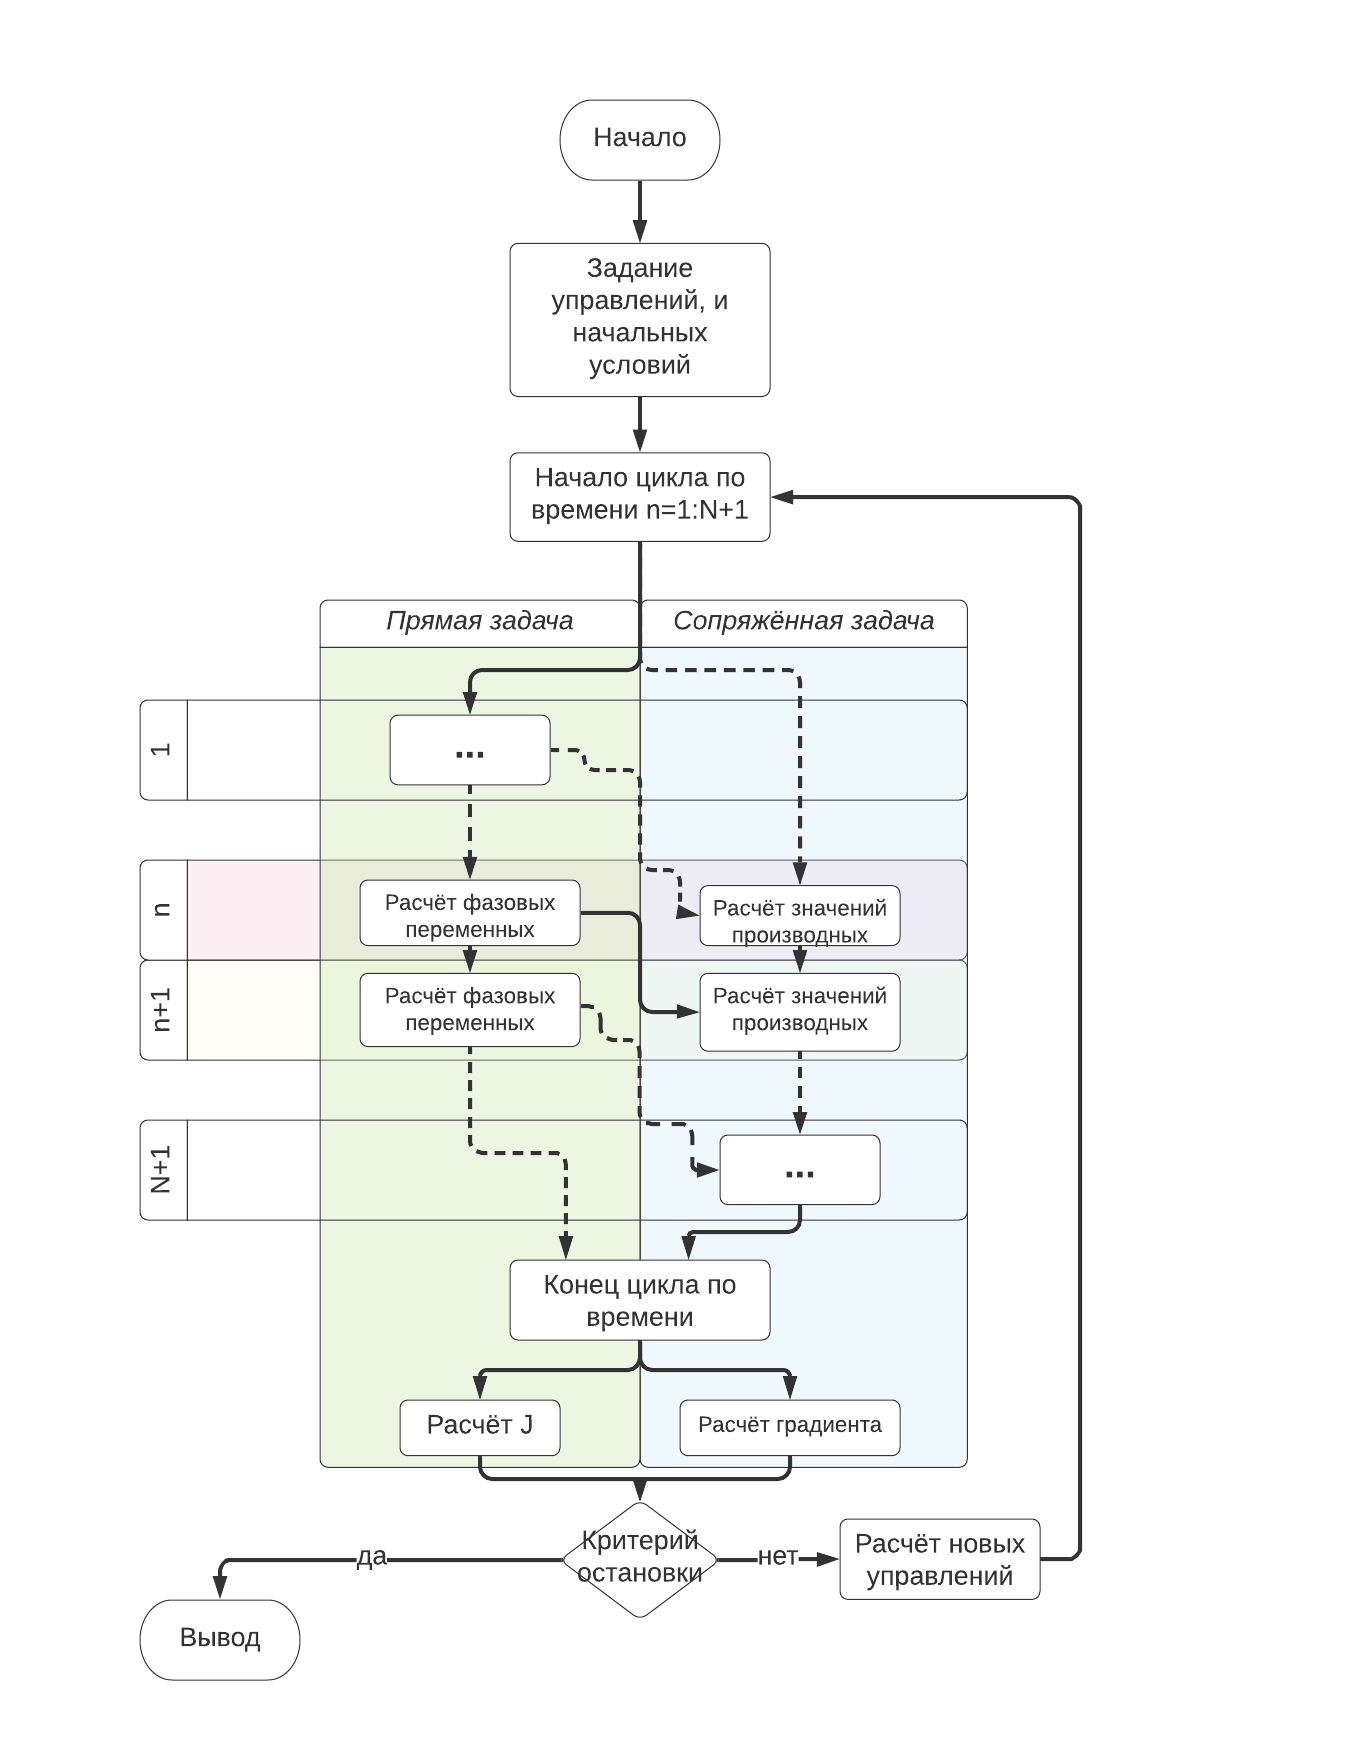
\includegraphics[width=24pc]{fig_chem.png}}
	\caption{Схема расчётов]}
	\label{fig:chem}
\end{figure}
На рисунке \ref{fig:chem} представлена принципиальная схема организации вычислительных процедур. Ввиду того, что решение сопряжённой задачи на каждом временном шаге зависит от решения прямой задачи, предлагается сместить процедуру расчёта сопряженной задачи на 1 шаг по времени. Таким образом в цикле по времени будет на 1 итерацию больше, но на последней итерации N+1, решение прямой задачи не происходит, а на первом шаге не решается сопряжённая задача. Подобная организация процесса вычисления в случае наличия нескольких вычислительных ядер позволяет масштабировать скорость вычисления практически пропорционально количеству вычислительных ядер. 
\section{Вычислительный эксперимент}
Для демонстрации работы представленного алгоритма проведём вычисления на синтетической модели нефтяного месторождения.

\section{Анализ производительности вычислений}
Сопоставление производительности вычислений представленного алгоритма можно провести с методом поиска градиента Лагранжа-Понтрягина
\newpage

\bibliographystyle{alpha}
\begin{thebibliography}{10}

	\bibitem{Kanevskaya2002} Каневская Р.Д. Математическое моделирование гидромеханических процессов разработки месторождений углеводородов. Институт компьютерных исследований, Москва-Ижевск, 2002 г., 140 стр., УДК: 532, ISBN: 5-93972-153-2

	\bibitem{Ashworth2019} Ashworth, M., Doster, F. Foundations and Their Practical Implications for the Constitutive Coefficients of Poromechanical Dual-Continuum Models. Transp Porous Med 130, 699–730 (2019). https://doi.org/10.1007/s11242-019-01335-6	
	
	\bibitem{Nguyen2010} Nguyen, V.X., Abousleiman, Y.N.: Poromechanics solutions to plane strain and axisymmetric mandel-type problems in dual-porosity and dual-permeability medium. J. Appl. Mech. 77(1), 011002 (2010)

	\bibitem{Barenblatt1960} Barenblatt, G., Zheltov, I., Kochina, I.: Basic concepts in the theory of seepage of homogeneous liquids in
fissured rocks [strata]. J. Appl. Math. Mech. 24(5), 1286–1303 (1960)	
	
	\bibitem{Warren1963} Warren, J., Root, P.J., et al.: The behavior of naturally fractured reservoirs. Soc. Petrol. Eng. J. 3(03), 245–255 (1963)
		
	\bibitem{Choo2015} Choo, J., Borja, R.I.: Stabilized mixed finite elements for deformable porous media with double porosity.
Comput. Methods Appl. Mech. Eng. 293, 131–154 (2015)

	\bibitem{Lim1995} Lim, K.T., Aziz, K.: Matrix-fracture transfer shape factors for dual-porosity simulators. J. Pet. Sci. Eng. 13(3–4), 169–178 (1995)
		
	\bibitem{Berryman2002} Berryman, J.G., Pride, S.R.: Models for computing geomechanical constants of double-porosity materials from the constituents properties. J. Geophys. Res. Solid Earth 107(B3), ECV 2-1–ECV 2-14 (2002)
	
	\bibitem{Khalili1996} Khalili, N., Valliappan, S.: Unified theory of flow and deformation in double porous media. Eur. J. Mech. A Solids 15(2), 321–336 (1996)
	
	 \bibitem {Glorot2011} Xavier Glorot, Antoine Bordes, Yoshua Bengio. Deep sparse rectifier neural networks. International Conference on Artificial Intelligence and Statistics (2011).
	
\end{thebibliography}



\end{document}
